\documentclass{standalone}
\usepackage{pgfplots}
\begin{document}
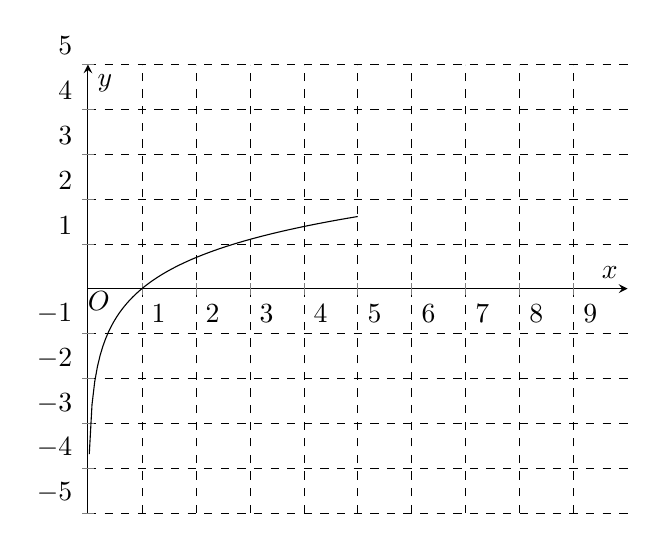
\begin{tikzpicture}
\begin{axis}
[
ymin=-5,ymax=5,
xmin=0,xmax=10,
%clip=false,
xtick=\empty,
ytick=\empty,
extra x ticks={1, 2, 3, 4, 5, 6, 7, 8, 9},
extra x tick labels={$1$, $2$, $3$, $4$, $5$, $6$, $7$, $8$, $9$},
extra y ticks={-5, -4, -3, -2, -1, 1, 2, 3, 4, 5},
extra y tick labels={$-5$, $-4$, $-3$, $-2$, $-1$, $1$, $2$, $3$, $4$, $5$},
every extra x tick/.style={
    xticklabel style={anchor=north west},
    grid=major,
    major grid style={very thin, dashed,black}
},
every extra y tick/.style={
    yticklabel style={anchor=south east},
    grid=major,
    major grid style={very thin, dashed,black}
},
axis lines = center,
xlabel=$x$,ylabel=$y$,
samples=200,
]
\addplot [black] {ln(x)};
\node at (axis cs:0.2, -0.28) {$O$} ;
\end{axis}
\end{tikzpicture}
\end{document}
